\section{Energy-Dependence of the Scattering Probabilities}
\label{sec:energyDepOfScatProbsAppendix}
A model for energy dependent scattering probabilities is derived. The expected amount of scatterings for a $\upbeta$ electron when travelling  through the whole \gls{wgts} volume of length $L$ filled with a gas of constant density $\rho$ is
\begin{equation}
    \mu(E,\thetaSource) =
    \frac{\sigma(E)\rho L}{\cos\thetaSource},
\end{equation}
where $E$ denotes the electron's kinetic energy; $\thetaSource$ the starting pitch angle; and $\sigma(E)$ the energy dependent scattering cross section.

The volume of the \gls{wgts} is divided into $N$ slices of equal width $w=L/N$. $N$ is chosen sufficiently large that the probability for a $\upbeta$ electron to scatter twice within one slice is essentially zero. Then, for large $N$ the probability to scatter within one slice is $\mu(E,\thetaSource)/N$. The probability not to scatter within $n$ slices is
\begin{equation}
    p_0(E,\thetaSource,n) =
    \left(
        1-\frac{\mu(E,\thetaSource)}{N}
    \right)^n
    \fullstop
\end{equation}
Using the well known limit for the Euler constant, one obtains for $n=N$ and $N\rightarrow\infty$ that $p_0$ is a Poisson distribution with expectation $\mu$ evaluated at 0 
\begin{align}
    \lim_{N\rightarrow\infty} 
    p_0(E,\thetaSource,N) =
    \lim_{N\rightarrow\infty} 
    \left(
        1-\frac{\mu(E,\thetaSource)}{N}
    \right)^N =
    \mathrm{e}^{-\mu(E,\thetaSource)}
    \fullstop
\end{align}
Assuming a constant energy loss per scattering of $\epsilon$ the probability to scatter $l$ times within $n$ slices can be expressed recursively
\begin{equation}
    p_l(E,\thetaSource,n) =
    \underbrace{
        \sum_{k=l}^{n}
    }_{(4)}
    \underbrace{
        p_{l-1}(E,\thetaSource,k-1)
        \vphantom{\sum_{k=l}^{n}}
    }_{(1)}
    \underbrace{
    \left(
        1-p_0(E-(l-1)\epsilon,\thetaSource,1)
    \right)
    \vphantom{\sum_{k=l}^{n}}
    }_{(2)}
    \underbrace{
        p_0(E-l\epsilon,\thetaSource,n-k)
        \vphantom{\sum_{k=l}^{n}}
    }_{(3)}
    \fullstop
\end{equation}
The terms have the following meaning:
\begin{enumerate}[(1)]
    \item Probability to scatter $l-1$ times within $k-1$ slices with a kinetic energy of $E$.
    \item Probability to scatter once within the $k$th slice with a kinetic energy of $E-(l-1)\epsilon$.
    \item Probability not to scatter within the remaining $N-k$ slices.
    \item Sum over all slices $k$. The sum starts at $l$ because the probability to scatter $l-1$ times within less than $k=l-1$ slices (term (1)) is 0.
\end{enumerate}
The probability to scatter $l$ times can be averaged over all starting positions. The averaging sum can be further approximated by an integral as this helps cutting down on run time in a numerical evaluation
\begin{equation}
    \label{eq:EnergyDepScatProbsAppendixZAverage}
    \bar{p}_l(E,\thetaSource) = 
    \sum_{\nSource}^{N} p_l(E,\thetaSource,\nSource) \approx
    \frac{1}{L}
    \int_{0}^{L}
        p_l(E,\thetaSource,
            \left\lceil N \frac{\zSource}{L}\right\rceil
        )
    \d \zSource
    \fullstop
\end{equation}
Then the limit $N\rightarrow\infty$ is applied
\begin{equation}
  P^{\star}_l(\Esource,\thetaSource) = 
    \lim_{N\rightarrow\infty} \bar{p}_l(\Esource,\thetaSource)
    \label{eq:energyDepScatProbsAppendix}
\end{equation}
$P^{\star}_l(\Esource,\thetaSource)$ denotes the probability for a $\upbeta$ electron to scatter $l$ times when travelling through the whole \gls{wgts} with a starting energy $\Esource$ and pitch angle $\thetaSource$ averaged over all starting positions. Finally, this expression has to be averaged over all starting pitch angles in order to obtain the energy dependent scattering probabilities
\begin{equation}
    \bar{P}^{\star}_l(\Esource) = 
    \frac{1}{1-\cos\thetaMax}
    \int_0^{\thetaMax}
        P^{\star}_l(\Esource,\thetaSource) 
        \d \thetaSource
    \fullstop
    \label{eq:averagedEnergyDepScatProbsAppendix}
\end{equation}

\subsection{Numerical Evaluation}
\label{sec:energyDepOfScatProbsAppendixNumEval}
\begin{figure}[t]
    \centering
    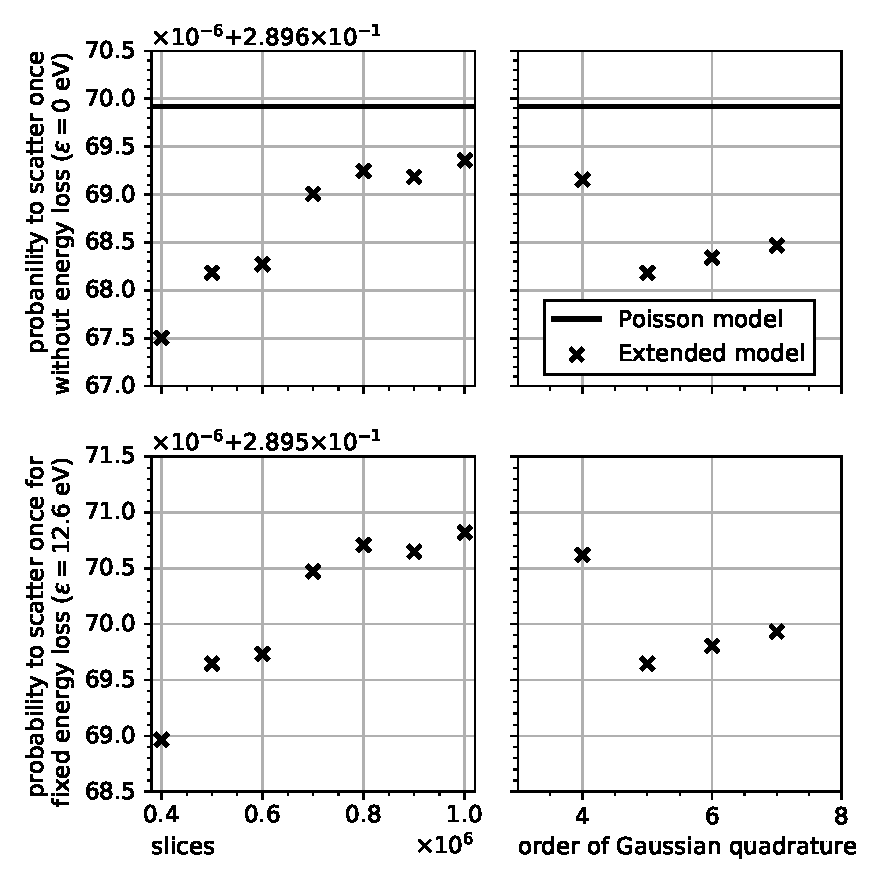
\includegraphics{chapter/energyDependentCrossSec/appendix/fig/scatProb1_numericalAccuracy.pdf}
    \xcaption{Numerical accuracy of the extended model for the scattering probabilities}{Numerical accuracy of the extended model for the scattering probabilities.}{The extended model is given by \eqref{eq:energyDepScatProbsAppendix}. The left column shows the dependence on the number of slices of the \gls{wgts}. The right column shows the order of Gaussian quadrature that was used to evaluate the two integrals in the model. For the left column the order of Gaussian quadrature was fixed to 5. For the right column the number of slices was fixed to $5\times10^{5}$. The upper row shows the extended model for no energy loss per scattering (markers). Its exact solution is given by the Poisson model (see \eqref{eq:energydepScatProbsPoissonModel}). The lower row shows the model for an energy loss of \SI{14.1}{eV} per scattering. The results make it plausible to assume a one-sided numerical inaccuracy on the $10^{-5}$ level for $N=10^5$ and using Gaussian quadrature of order 5.}
    \label{fig:scatProb1NumericalAccuracy}
\end{figure}
The energy dependent probability to scatter once $\bar{P}^{\star}_1$ in \eqref{eq:averagedEnergyDepScatProbsAppendix} was evaluated numerically. In \eqref{eq:energyDepScatProbsAppendix} taking the limit $N\rightarrow\infty$ was replaced by choosing a large $N$. The averaging integral over the starting positions \eqref{eq:EnergyDepScatProbsAppendixZAverage} and pitch angles \eqref{eq:averagedEnergyDepScatProbsAppendix} was computed using Gaussian quadrature. 

Figure \ref{fig:scatProb1NumericalAccuracy} shows the result in dependence of $N$ and the order of the Gaussian quadrature. Both should be chosen as low as possible to cut down on run time but sufficiently high for the required accuracy. As a cross check, for an energy loss of $\epsilon=\SI{0}{eV}$ per scattering, the suggested extended model \eqref{eq:averagedEnergyDepScatProbsAppendix} must recover the Poisson model (see \eqref{eq:energydepScatProbsPoissonModel}). For $N=10^6$ and using Gaussian quadrature of order 5, they differ approximately $3\times10^{-6}$. Furthermore, the numerical calculation converges from below, which can be interpreted as a one-sided numerical inaccuracy. The calculations for $\epsilon=\SI{14.1}{eV}$ are shown in the lower row of figure \ref{fig:scatProb1NumericalAccuracy}. They also show convergence on the $10^{-5}$ level. Conclusively, the results make it plausible to assume a one-sided numerical inaccuracy on the $10^{-5}$ level for $N=10^5$ and using Gaussian quadrature of order 5 for the integrals.

The corresponding run time to compute $\bar{P}^{\star}_1$ is in $\mathcal{O}(N)$ as it requires a sum over all $N$ slices. Note that the extended model is defined recursively and therefore, the run time for $l$-fold scattering is in $\mathcal{O}(N^l)$. Hence, computing the probability for 2-fold scattering would take 500000 times as long as for 1-fold scattering for the same $10^{-5}$ accuracy. This was found not to be feasible. For 2-fold scattering $N=5000$ and also Gaussian quadrature of order 5 was chosen for a numerical accuracy on the $10^{-3}$ level.